%% report.tex
%% 16 March 2015
%% by Matthew Stone and Stephen Malina

\documentclass[10pt,conference]{IEEEtran}

\usepackage[cmex10]{amsmath}
\usepackage{cite}
\renewcommand{\citedash}{--}% Default is ]--[
\renewcommand{\citepunct}{, }% Default is ], [

% \usepackage{algorithm}
% \usepackage[noend]{algpseudocode}
% \usepackage{array}
\usepackage{textcomp}
\usepackage{url}

\usepackage[pdftex]{graphicx}
\graphicspath{{./figures/}}
\DeclareGraphicsExtensions{.pdf,.jpg,.png}

\usepackage[caption=false,font=footnotesize]{subfig}

\newcommand{\vocab}[1]{\textit{#1}}

\begin{document}

\title{A Modern Implementation of the \\
Basic Immune Simulator}

\author{\IEEEauthorblockN{Matt Stone, Stephen Malina}
\IEEEauthorblockA{Department of Computer Science\\
Dartmouth College}}

\maketitle
\thispagestyle{plain}
\pagestyle{plain}

\section{Introduction}
\noindent
Characterizing the complex behavior of the adaptive and innate immune systems
is essential for developing treatments for bacterial, fungal, and parasitic
infections. In particular, the innate immune system response contributes to
immunity to these infections and plays a role in diseases such as
atherosclerosis, lung fibrosis, asthma, and sepsis. As a result, models of
these systems will allow researchers to generate hypotheses for the origins of
disease and possible treatments for these diseases~\cite{Folcik:2007}. Folcik
et al.\ presented the Basic Immune Simulator (BIS) as an initial foray into
this realm of hypothesis genesis. We proposed an updated implementation of the
BIS, capable of performing on modern computers and accounting for some of the
observed shortcomings in the original.  We chose to limit our implementation to
the innate immune system in order to isolate and better characterize its
behavior, as opposed to the interplay between the two systems.

\indent
We used an agent-based model for our simulation, basing our implementation off
the defined agent types in Folcik's paper. In Folcik's agent-based model,
agents represent immune cells of different types, emitting signals which
represent the intercellular communication that occurs \textit{in-vivo}. Folcik
et al.\ chose to operate at this level of abstraction because it provides the
best combination of understandability and accuracy. The cell represents a
well-defined, well-characterized unit of abstraction~\cite{Folcik:2007}.

\indent
We intended for our updated BIS simulation to narrow the scope of the original
BIS in order to allow users to better understand and modify its behavior. We
improved upon the original BIS in a number of ways. First, we modified the
behavior of portal cells and their activation of MP and NK cells. Our portal
cells are located in open space, away from PCs and release MP and NK cells upon
detection of PC stress signals. This modification creates a delay between
viral infection and innate immune system response. Second, we modified PC cell
viral emission and infection thresholds to generate a more gradual infection
and response. Third, we added behavior to parenchymal cells that represents
bursting with the virus after an incubation period. Our focus on the innate
immune system, however, trivially eliminated the hyper-response observed in the
original BIS and prevented an adequate analysis of its cause.

\vspace{.5in}
\section{Methods}
\subsection{Development}
The updated version of the BIS was created using Python and visualized using
matplotlib~\cite{Hunter:2007}, a Python library with functionalities for graph
display and animation.

\indent
Each agent of the model consists of a Python class that encodes the state
machine defined in the original BIS~\cite{Folcik:2007}. Agent behaviors result
from changes in state triggered by the detection of specific levels of signals
or the presence of various agents.  Transition rules, composed of logical
statements that measure signal values and check for the presence of different
types of agents represent the interaction of the cell with its surrounding
environment. The overall behavior of the system results from these individual,
local interactions.

\subsection{Simulation Agents}

\begin{figure*}[h]
% \begin{figure*}
\centering
\captionsetup{justification=centering,width=7.0in}
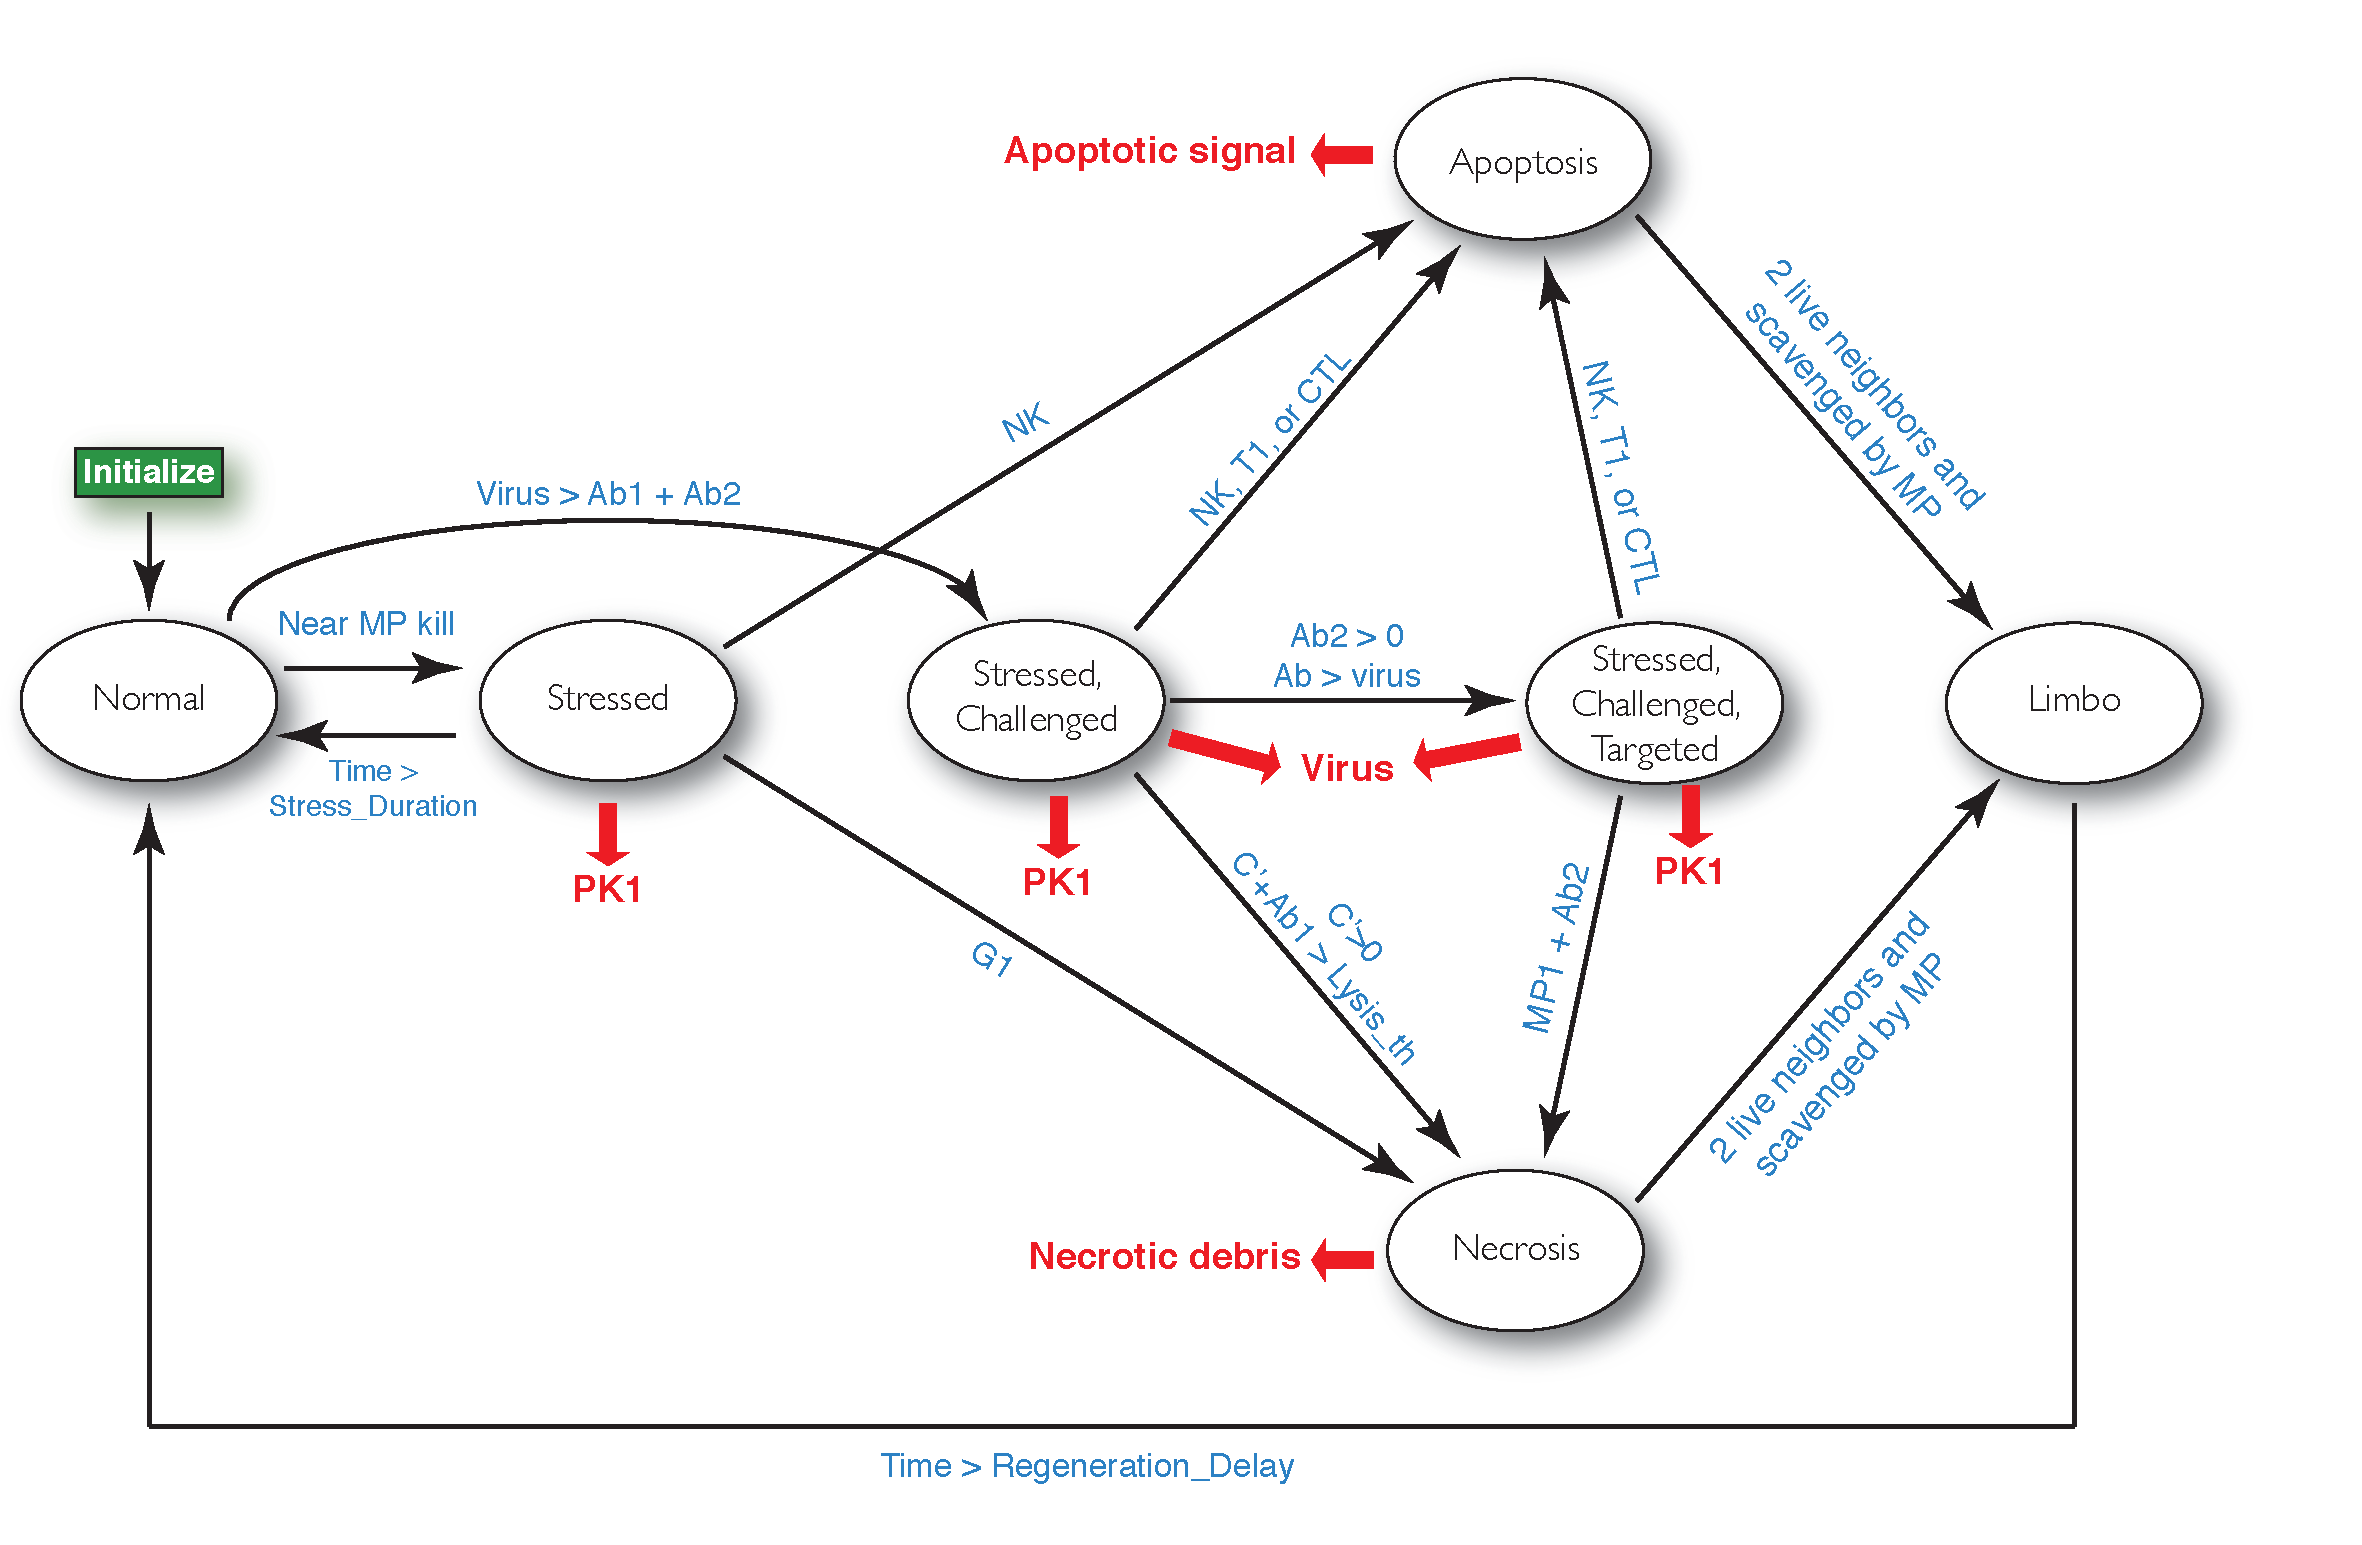
\includegraphics[width=7in]{PC_fsm}
% \includegraphics[width=\textwidth]{Parenchymal_Cell_State_Machine}
\caption{Parenchymal Cell state machine. Shows the state transition rules for
    the PC\@. As shown, the PC can either be Stressed: it detects virus signal,
    Challenged (infected), Apoptotic: it's been killed by an NK cell, Necrotic:
    it's been killed by a macrophage, or in Limbo: it's waiting to regenerate
    for a specified number of ticks.}
\label{PC_fsm}
\end{figure*}
% \end{figure*}
Rather than trying to replicate every type of cell in the immune system, we
focused on the primary cells of the innate immune system: macrophages (MP),
natural killer (NK) cells, and parenchymal (tissue) cells. We also limited our
signals to two signals (an upregulating signal and a downregulating one) for
each immune cell, and limited the parenchymal cell to stress, apoptotic,
necrotic, and virus signals as seen in Figure~\ref{PC_fsm}. This simplification
allows us to modulate the behavior of our system by changing the values of a
few parameters.

Cells, modeled as agents in the updated BIS, model both functional tissue and
the cells of the innate immune system. Cells can probe their Moore neighborhood
-- the 8 cells in their immediate vicinity and the one they are in -- and
detect agents and cells within it. Cells that can move begin by moving randomly
before discovering signals whose gradients they are programmed to follow.

\indent
Parenchymal cells represent functional tissue. These cells get infected and
release stress and virus signals, spreading the infection and signaling their
own status. These cells cannot move and are surrounded by up to 6 other
cells of their own kind. They regenerate after a certain amount of time once
they have been scavenged by macrophage cells. The updated BIS adds an infection
incubation period, during which the infected parenchymal cell releases no virus
signal. Upon conclusion of this period, the parenchymal cell releases a burst
of virus signal. The behavior of parenchymal cells is detailed in
Figure~\ref{PC_fsm}.

\indent
The updated BIS uses macrophages and natural killer cells to model the activity
of the innate immune system. Macrophages perform dual function: infected cell
destruction and scavenging. These cells follow chemical gradients of PC signal
emissions in order to find infected, apoptotic, and necrotic PC cells, killing
or scavenging them. Natural Killer cells can only kill PC cells, also following
the chemical gradients of PC cells' various signals.

\indent
Certain agents possess input parameters that determine their lifespan. These
parameters are, in some cases, modified by specific state transition.

\subsection{Simulation Zones}
The original BIS used three "zones" of cell activity to represent different
areas in the body where cell interactions occur. These three zones represented
functional tissue, the lymph nodes, and the circulatory system
respectively~\cite{Folcik:2007}. Our implementation incorporates only a single
zone representing generic tissue.  This zone uses the same geometric
configuration as the zones in the original BIS do, a torus, represented as a
two-dimensional grid that permits travel from one edge to the opposing edge.
The updated BIS zone has dimensions of 20x20. The zone used represents a small
slice of tissue, only large enough to allow the virus to take hold and spread.
Exact zone size was selected so as to allow the simulation to run for a
reasonable (more than 100 ticks) length in a reasonable amount of time (under
one minute).

\indent
Unfortunately, since the number of immune cells that react to pathogens is both
unknown and not easily translatable to this model, initial cell counts were
selected arbitrarily in order to produce the desired simulation response. Agents are
released from storage cells, called Portals, when the portals detect PC stress
signal (PK1) in the single cell that they monitor. This behavior simulates the
movement of innate immune cells in to stressed functional tissue in the body in
response to a foreign pathogen.

\subsection{Signal Diffusion and Time}
The updated BIS uses the same model of "ticks" and signal diffusion as the
original BIS~\cite{Folcik:2007}. Signals diffuse into the surrounding
environment fairly rapidly as a result.

\section{Results and Discussion}
\noindent
We successfully implemented agents simulating parenchymal cell, macrophage, and
natural killer cell behavior, adhering to the finite state machines defined by
Folcik et al.~\cite{Folcik:2007}. A successful response neutralizing the viral
infection can be seen in Figure~\ref{sim_screen}, and a video of the full
simulation is attached as supplementary material. 

Unfortunately, our simulation was limited by the constraints we imposed on the
implementation. Both macrophages and natural killer cells are generated from
portal cells at the same location and are created simultaneously, and are
programmed to follow the same chemical gradient (PK1). This behavior is the
defined behavior for natural killer cells in the original paper, but
macrophages were originally permitted to follow cytokine-1, complement,
necrotic debris, apoptotic, or antigen-antibody complex signals by Folcik et
al.~\cite{Folcik:2007}. Of these, only necrotic debris and apoptotic signal
were present in our implementation. Folcik et al.\ did not specify the priority
each signal should take when both were encountered, and since necrotic debris
and apoptotic signal can only originate from a formerly stressed cell we
assumed that their gradients would correlate with PK1 regardless. The
consequence of this is that natural killer cells and macrophages cohabitate
spaces on the grid for the entirety of their existence, and it is impossible to
examine the interaction of either independently. We experimented with random
motion around the zone, but this led to sustained viral infection overwhelming
the zone's parenchymal cells. 

We encountered difficulties adequately capturing immune system behavior. This
was due in part to our naive simplifications of Folcik et al.'s model, but also
due to poorly defined parameterization in the original paper. Initial viral
load, how the virus signal behaves relative to intracellular signaling
molecules, behavior of infected cells in emitting viral signal, and strength of
emitted signal were all left undefined by Folcik et al. We also found a number
of parameters referenced that made no appearance in the defined state machines. 

Despite our hope to expand the size of the simulated tissue beyond the
original's 100x100 grid, we were forced to confine ourselves to testing in a
20x20 grid. We recorded a simulated response in a 100x100 grid in an early
implementation, but it ran for several hours before crashing. A video of the
saved portion of the simulation is attached as supplementary material.

We found that the behavior of our simulator was extraordinarily sensitive to
the settings of the initial parameters, particularly the initial viral load and
the strength and frequency of viral signal emitted by infected parenchymal
cells. Despite these parameters being fundamental to the accuracy of the
simulator, we could not find a definition provided by Folcik et al. We conclude
that while simulation may play a useful role in hypothesis generation, its
behavior depends heavily on the assumptions made and the experimental knowledge
of the simulated system.

\begin{figure*}[h]
\centering
\captionsetup{justification=centering,width=7.0in}
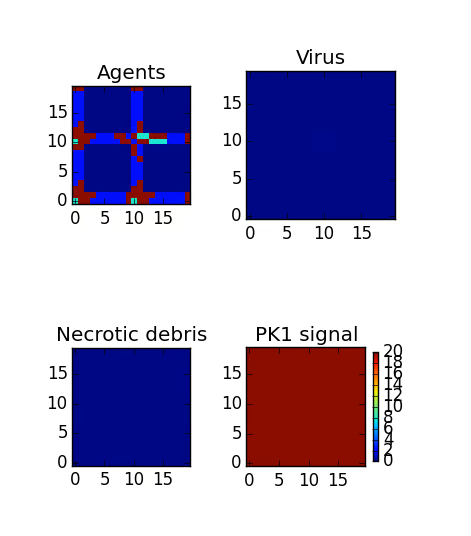
\includegraphics[width=7in]{sim_screenshot}
\caption{Simulated innate immune response to a viral signal. Upper left) The
    cells present in the infected tissue. Parenchymal cells appear in a static
    grid. Blue cells are healthy but may be stressed, red cells are infected,
    and dark brown cells are dead. Macrophage cells are yellow if inactive and
    grey if active. Natural killer cells are orange. Upper right) Density of
    viral signal. Lower left) Density of necrotic debris signal. Lower right)
    Density of PK1 (parenchymal cell stress) signal.}
\label{sim_screen}
\end{figure*}

As far as division of labor, Stephen proposed the project after presenting the
original BIS paper in class. We jointly discussed which agents to prioritize.
Stephen drafted the original agent class and FSM implementation, while Matt
wrote the initial animation code. We worked as a pair to debug both the agent
and animation and extend the functionality of the Zone. We collaborated on
tweaking infection and response parameters to adjust the immune response.

\bibliographystyle{IEEEtran_etalRoman}
\bibliography{refs.bib}

\end{document}
